% Created 2020-06-30 Tue 07:07
% Intended LaTeX compiler: pdflatex
\documentclass[11pt]{article}
\usepackage[utf8]{inputenc}
\usepackage[T1]{fontenc}
\usepackage{graphicx}
\usepackage{grffile}
\usepackage{longtable}
\usepackage{wrapfig}
\usepackage{rotating}
\usepackage[normalem]{ulem}
\usepackage{amsmath}
\usepackage{textcomp}
\usepackage{amssymb}
\usepackage{capt-of}
\usepackage{hyperref}
\usepackage{color}
\usepackage{listings}
\usepackage[table,xcdraw]{xcolor}
\usepackage{listings}
% src: http://texdoc.net/texmf-dist/doc/latex/listings/listings.pdf
% c/c++
\lstdefinestyle{customc}{
  belowcaptionskip=1\baselineskip,
  breaklines=true,
  %frame=L,%lines, whole
  xleftmargin=\parindent,
  language=C,
  showstringspaces=false,
  basicstyle=\scriptsize\ttfamily,
  keywordstyle=\bfseries\color{green!40!black},
  commentstyle=\itshape\color{purple!40!black},
  identifierstyle=\color{blue},
  stringstyle=\color{orange},
  numberstyle={\tiny},
  numbers=left,
  numberblanklines=false,
  stepnumber=5,
  backgroundcolor=\color{yellow!10}, 
  frame=tlb
}
\lstset{escapechar=@,style=customc}
% ASM
\lstdefinestyle{customasm}{
  belowcaptionskip=1\baselineskip,
  frame=L,
  xleftmargin=\parindent,
  language=[x86masm]Assembler,
  basicstyle=\footnotesize\ttfamily,
  commentstyle=\itshape\color{purple!40!black},
}
% MATLAB: src: https://tex.stackexchange.com/a/75124
\definecolor{greenmb}{RGB}{28,172,0} % color values Red, Green, Blue
\definecolor{lilasmb}{RGB}{170,55,241}
\lstdefinestyle{custom-matlab}{
  % \lstset{language=Matlab,%
  language=Matlab,
    %basicstyle=\color{red},
    breaklines=true,%
    morekeywords={matlab2tikz},
    keywordstyle=\color{blue},%
    morekeywords=[2]{1}, keywordstyle=[2]{\color{black}},
    identifierstyle=\color{black},%
    stringstyle=\color{lilasmb},
    commentstyle=\color{greenmb},%
    showstringspaces=false,%without this there will be a symbol in the places where there is a space
    numbers=left,%
    numberstyle={\tiny \color{black}},% size of the numbers
    numbersep=9pt, % this defines how far the numbers are from the text
    emph=[1]{for,end,break},emphstyle=[1]\color{red}, %some words to emphasise
    %emph=[2]{word1,word2}, emphstyle=[2]{style},    
}
% Java: src: 
\lstdefinestyle{custom-java}{
	language=Java,
	tabsize = 4, %% set tab space width
	showstringspaces = false, %% prevent space marking in strings, string is defined as the text that is generally printed directly to the console
	numbers = left, %% display line numbers on the left
	commentstyle = \itshape\color{purple!40!black}, %% set comment color
	keywordstyle = \bfseries\color{green!40!black}, %% set keyword color
	identifierstyle=\color{blue},
	stringstyle = \color{orange}, %% set string color
	rulecolor = \color{black}, %% set frame color to avoid being affected by text color
	basicstyle = \footnotesize\ttfamily , %% set listing font and size
	breaklines = true, %% enable line breaking
	numberstyle = \tiny,
	stepnumber=1,
	xleftmargin=\parindent,
	backgroundcolor=\color{yellow!10}, 
    frame=L,
}

\author{José Miguel Alves Pires\thanks{a50178@alunos.uminho.pt}}
\date{\textit{<2020-06-30 Tue>}}
\title{cheatsheet}
\hypersetup{
 pdfauthor={José Miguel Alves Pires},
 pdftitle={cheatsheet},
 pdfkeywords={},
 pdfsubject={},
 pdfcreator={Emacs 26.3 (Org mode 9.3.6)}, 
 pdflang={English}}
\begin{document}

\maketitle
\tableofcontents


\section{Modular design\hfill{}\textsc{Important}}
\label{sec:org400fc2f}
Modular design is useful to separate logical units inside the \LaTeX{} environment.
\begin{itemize}
\item \texttt{dissertation.tex}: main document that defines all the formatting and includes
all the relevant \texttt{.tex} documents
\item \texttt{./sty}: contains the stylesheets for the document, such as:
\begin{itemize}
\item \texttt{dissertation-xelatex.sty}: stylesheet for the main document
\item \texttt{listing.sty}: stylesheet for the listings to be formatted and presented
\end{itemize}
\item \texttt{./sec}: contains secondary files, like images, PDFs, acronyms and symbols
\item \texttt{./bib}: contains the bibliography database
\item \texttt{./listing}: contains the listings (code) to be displayed
\item \texttt{./font}: contains the fonts to be used
\item \texttt{./tex}: contains the \texttt{.tex} documents to be inputted, subdivided in:
\begin{itemize}
\item \texttt{Pre\_Chap}: Pre chapters (not used here)
\item \texttt{Chap}: chapters
\item \texttt{Append}: appendices
\end{itemize}
\end{itemize}

Regarding \texttt{.tex} documents, they can be included as follows (the extension
\texttt{.tex} is implicit):
\begin{itemize}
\item \texttt{\textbackslash{}input\{path/to/file\}}: inputs the file as is (\textsubscript{recommended}\_)
\item \texttt{\textbackslash{}include\{path/to/file\}}: inputs the file and adds an extra blank page at the
end.
\end{itemize}

\section{Styling guides\hfill{}\textsc{Important}}
\label{sec:orga642a07}
\begin{enumerate}
\item Don't use \texttt{\textbackslash{}newpage}, \texttt{\textbackslash{}clearpage}, or any other section break command. This
is done natively by the \TeX{} engine; it should be done last and only if REALLY
required
\item To separate paragraphs use one blank line; any additional blank lines MUST BE
AVOIDED anywhere in the document. If you want to separate anything visually,
use a comment \texttt{\%}.
\begin{itemize}
\item Example:
\lstset{language=[LaTeX]TeX,label= ,caption= ,captionpos=b,numbers=none}
\begin{lstlisting}
%
\section{Product concept}%
\label{sec:product-concept}
%\section{Product concept}%
%\label{sec:orge7b0dc6}
The envisioned product consists of a remote controlled vehicle used to assist
exploration and maintenance domains, hereby, denominated as Radio Frequency
Camera Assisted Rover (RFCAR). To satisfy such requirements, the vehicle must
contain a remotely operated camera that provides a live video feed to the user.
Additionally, the vehicle must include an odometric system that assists the
driving and avoids unintentional collisions when remote control is compromised, e.g., when connection is lost.
The vehicle provides means for exploration and conditions assessment in critical
or unaccessible areas to human operators, such as fluid pipelines and other hazardous locations.
%
%%% Local Variables:
%%% mode: latex
%%% TeX-master: "../Phase1"
%%% End:

%
\section{Foreseen specifications}%
\label{sec:fores-spec}
\section{Foreseen product specifications}%
\label{sec:org31f7574}
In this section the foreseen product specifications of the system to be developed are provided. Such specifications were obtained through the intersection of customer, functional requirements and project restrictions.
\subsection{Quality Function Deployment}%
\label{sec:qfd}
The customer requirements are usually abstract and can collide with the functional requirements, compromising the fulfilment of the project. Thus, it raises the need of a methodology which converts abstract requirements into a series of concrete engineering specifications.

An efficient quality assessment methodology is the use of a Quality House (QFD). In this method, the desired requirements are laid out as rows and the engineering specifications/restrictions as columns. In the intersections lies a symbol representing the strength (weak, moderate or strong --- Figure~\ref{fig:QFD-R} ) of the relationship requirement-specification. This symbol is one of the many tools that allow the quantification of relations existing between the customer requirements and engineering specifications.
For instance, the `engine power' specification and the `fast' requirement have a
very strong correlation (9) since the power of the engine is directly
responsible for the speed of the car.

Along with the requirements, the importance given to each is also specified, ranging from 1 (lowest importance) to 5 (highest importance) these, along with the number at each intersection, will be used to calculate the importance of each specification and thus assign priorities for the Design Team.

Lastly, the triangle shape (the `roof' within the house metaphor) serves as another way of measuring relationships, this time between each specification: such is achieved by placing a symbol (ranging from very negative to very positive, see Figure~\ref{fig:QFD-Roof}) in the diagonal intersection of two specifications. 
I.e., the battery life will have a very negative correlation with the battery temperature, due to the fact that the increase of the temperature will cause a decrease in life time. As such a `very negative' correlation was placed in the diagonal intersection betwixt `Battery Life' and `Battery Temperature'. 
\begin{figure}[!htbp]
   \centering
       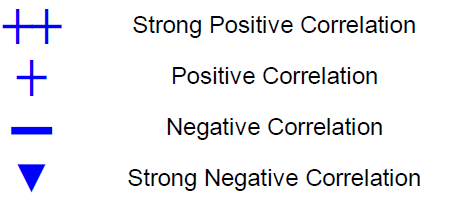
\includegraphics[page=1,width=0.5\textwidth]{sec/img/Roof_Symbols.png} 
 \caption{Quality House - Specification Correlation Strength Symbols}%
\label{fig:QFD-Roof}
\end{figure}

Figure~\ref{fig:QFD} shows the `Quality House' for the RF CAR containing:
\begin{itemize}
\item \textbf{Customer Requirements}: Vehicle Integrity; Obstacle Avoidance; Reliable Feedback; Fast Response; Fast; Budget Friendly; Low Consumption; Small.
\item \textbf{Functional Requirements or Restrictions}: Autonomy; Battery Temperature; Minimum Distance to Obstacle; Maximum Velocity; Motor Expectancy; Cost of Production; Motor Power; Ramp-Up Speed Time; Frame Rate; Camera Range; Resolution; Communication Range; Communication Speed; Dimensions; Mass.
\item \textbf{Intersection Values} (referencing the strength of the requirement-specification correlation) --- see Figure~\ref{fig:QFD-R}.
\item \textbf{Analytical Data}, depicting, in a quantifiable manner, the aims of the project and the relevance of each
  entity:
  \begin{itemize}
  \item Target or Limit Value: The metrics the design team will be based on, white spaces are left for either further discussion and refinement.
  \item Difficulty: Allows a subjective input to be added so that `importance' can be changed to balance unforeseen circumstances.
  \item Importance and Relative Weight: The main conclusion for which the QFD was used, it assigns the priorities for the design team in an objective manner.
  \end{itemize}
\end{itemize}
%
\begin{figure}[!htbp]
   \centering
       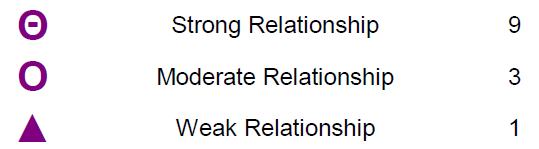
\includegraphics[page=1,width=0.5\textwidth]{sec/img/Relationship_Symbols.png} 
 \caption{Quality House - Relationship Strength Symbols}%
\label{fig:QFD-R}
\end{figure}
%
\begin{sidewaysfigure}[!htbp]
   \centering
       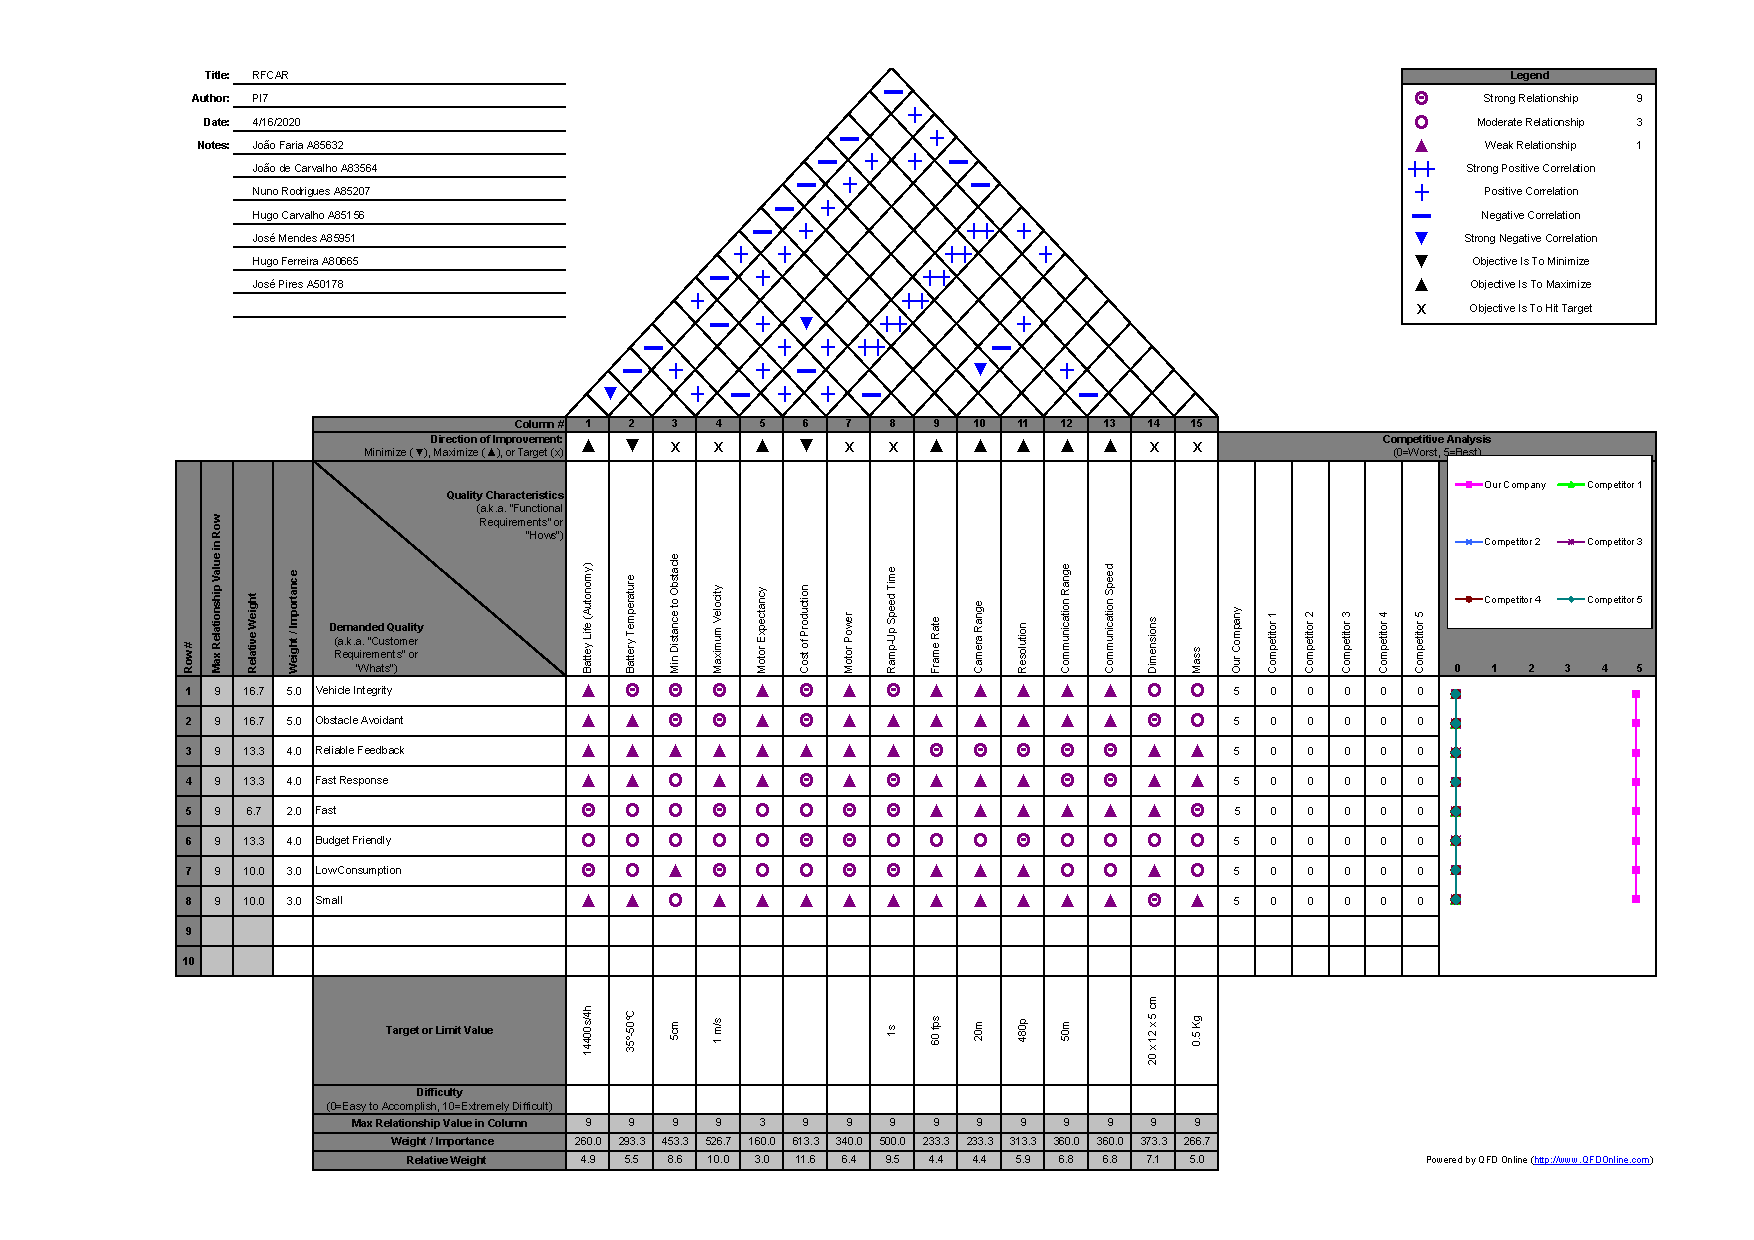
\includegraphics[page=1,width=1.0\textwidth]{sec/pdf/QFDv3.pdf} 
 \caption{Project Study --- RFCar Quality House}%
\label{fig:QFD}
\end{sidewaysfigure}
%
With the QFD, the prioritized ranks and specification targets were obtained and diffused within the Design Team with a
straightforward guideline. For instance, the low cost requirement should be
prioritized over all other specifications, followed by the maximum speed,
Ramp-Up Speed Time and so on.  On the other hand, the engine expectancy is of
little to no consequence (note that the importance added up to a mere 3\%),
followed by the camera-related specifications. This could be regarded as
a point of discussion, which should be prioritized? The functionality of the car
or the the feedback provided by the camera?

With the last point in mind, the QFD has the advantage of promoting further
discussion, simply by changing the importance of a requirement the priority ranking will change, ergo
the priorities can be altered, easily and efficiently, if deemed appropriate.
\newpage
%
\subsection{Vehicle Autonomy}%
\label{sec:autonomy-specs}
The vehicle is operated in wireless mode, thus, a portable power source must be included. The autonomy refers to the vehicle operating hours since the battery is fully charged and safely discharged and should be observed for the following scenarios:
\begin{itemize}
\item No load and vehicle operating at maximum speed;
\item No load and vehicle operating at mean speed;
\item Maximum load and vehicle operating at maximum speed;
\item Maximum load and vehicle operating at mean speed.
\end{itemize}
\subsection{Speed}%
\label{sec:speed-tests}
The vehicle must be operated within a safe range of speed, while also not increasing excessively the power consumption. Thus, these speed boundaries should be tested in the absence of an external load and in the presence of the maximum load.
\subsection{Safety}%
\label{sec:org83942c3}
Vehicle self integrity protection is a requirement in product design, especially considering the vehicle is to
be remotely operated. The safety in the operation can be analysed in two ways, and considers the
preservation of people and goods. For the former, it is important to assure safe interaction as well as user operation --- the vehicle may encounter
several obstacles along its path, but it must not inflict any damage. For the
latter, the vehicle under operating conditions must not inflict any damage to
goods. Thus, in the presence of conflicting user commands violating the safety
of people and goods, the local system should override them, taking corrective
measures to prevent it. The same holds true if the communication between user
and system is lost.
%The system uses odometric navigation.
%\item Human: Due to the odometric sensors safely fixed in the car, crashes will not occur, making it much harder for the car to hit a person or for any part of the car to jump and cause harm to the user or anyone around.
%\end{itemize}
\subsection{Image acquisition}%
\label{sec:image-acquisit}
The vehicle is equipped with a camera to assist in its navigation,
thus, requiring it to be fed to the user's platform appropriately. To do so, several functionalities details need to be addressed efficiently. It was selected the most relevant three and these include the frame rate, the resolution and the image range.
\subsubsection{Frame rate}%
\label{sec:org5adf4ee}
Frame rate refers to the frequency at which independent still images appear on the screen. A better image motion is the result of a higher frame rate but the processing overhead increases as well, so a compromise must be achieved between the quality of the image and the increased processing overhead required. The minimum frame rate defined must be such that allows a clear view of the navigation.
\subsubsection{Range}%
\label{sec:orgecb044c}
How far can the camera capture images without being distorted or unseen by the user. The range must be such that allows the user to see the obstacles when the car is heading to them and provide enough time to change the direction.
\subsubsection{Resolution}%
\label{sec:orgba87554}%
The amount of detail that the camera can capture. It is measured in pixels. The quality of the acquired image is proportional to the number of pixels but a increased resolution requires a greater data transfer and processing overhead, thus, a compromise must be achieved. The minimum resolution must be such that provides the least amount of information required for the user. 
\subsection{Communication}%
\label{sec:org4241610}
For the implementation of the communication, several stages must be considered: Reliability, redundancy and communication range.
\subsubsection{Reliability}%
\label{sec:orgdcb920d}	
A communication is reliable if it guarantees measures to deliver the data
conveyed in the communication link. As reliability imposes these measures, it
also increases memory footprint, which must be considered
depending on the case. For the devised product, an user command
must be acknowledged to be processed, otherwise, the user must be informed; on
the other hand, loosing frames from the video feed is not so critical — user can
still observe conveniently the field of vision if the frame rate is within
acceptable boundaries.
\subsubsection{Redundancy}
\label{sec:orgc5933fc}
The communication protocols are not flawless and the car relies on them to be controlled. If the communication is lost, the car cannot be controlled. A possible solution for this issue is using redundancy in the communication protocols (e.g Wi-Fi and GPRS), so if one protocol fails, the car will still be controlled using the other.
\subsubsection{Range}%
\label{sec:org447a205}
The communication protocols have a limited range of operation, and, as such, regarding the environment on which the car is used the range can be changed.
The range established the maximum distance allowed between user and system for communication purposes.
\subsection{Responsiveness}%
\label{sec:org622e63a}
The movement of the car will be determined by the tilt movement of the smartphone. Sensibility refers to the responsiveness of the car on the minimum smartphone tilt movement. The sensibility must be in an range of values in which small unintentional movements will not be enough to change the state of the car and it does not take big smartphone tilts for the car to move.
\subsection{Closed loop error}%
\label{sec:closed-loop-error-specs}
The speed, direction and safe distance to avoid collisions must be continuously monitored to ensure proper vehicle operation. The closed loop error must then be checked mainly in three situations as a response to an user command:
\begin{itemize}
\item speed: the user issued an command with a given mean speed, which should be compared with the steady-state mean speed of the vehicle.
\item direction: the user issued an command with a given direction, which should be compared to the vehicle direction.
\item safe distance to avoid collisions: the user issued an command with a given direction and speed which can cause it to crash. The local control must influence, to prevent collision, and the final distance to the obstacles must be assessed and compared to the defined one.
\end{itemize}
\subsection{Summary}%
\label{sec:org1f95256}
Table~\ref{tab:specs-init} lists the foreseen product specifications.

% Please add the following required packages to your document preamble:
% \usepackage[table,xcdraw]{xcolor}
% If you use beamer only pass "xcolor=table" option, i.e. \documentclass[xcolor=table]{beamer}
% Please add the following required packages to your document preamble:
% \usepackage[table,xcdraw]{xcolor}
% If you use beamer only pass "xcolor=table" option, i.e. \documentclass[xcolor=table]{beamer}
\begin{table}[!hbt]
\centering
\caption{Specifications}%
\label{tab:specs-init}
%
\begin{tabular}{
>{\columncolor[HTML]{FFFFFF}}l 
>{\columncolor[HTML]{FFFFFF}}l 
>{\columncolor[HTML]{FFFFFF}}l }
\hline
                  & Values     & Explanation                                                                                                  \\ \hline
Autonomy          & 4 h        & \begin{tabular}[c]{@{}l@{}}Time interval between battery fully \\ charged and safely discharged\end{tabular} \\ \hline
Speed Range  & 0.1 to 1 m/s    & \begin{tabular}[c]{@{}l@{}}Speed at which the car can operate\end{tabular}              \\ \hline
Frame Rate        & 60 fps     & \begin{tabular}[c]{@{}l@{}}Frequency at which independent still \\ images appear on the screen\end{tabular}  \\ \hline
Camera Range      & 20 m       & \begin{tabular}[c]{@{}l@{}}How far can the camera capture images\\ without loosing resolution\end{tabular}   \\ \hline
Camera resolution & 480p       & Amount of detail that the camera can capture                                                                 \\ \hline
Communication Range & 50 m & \begin{tabular}[c]{@{}l@{}}Maximum distance between the car and the\\ smarphone without losing connection\end{tabular} \\ \hline
speed Error    & 5 \%       & \begin{tabular}[c]{@{}l@{}}Maximum difference between desired \\ and real speed\end{tabular}              \\ \hline
Direction Error   & 5\%        & \begin{tabular}[c]{@{}l@{}}Maximum difference between desired\\  and real direction\end{tabular}             \\ \hline
Distance Error     & 5 \% & \begin{tabular}[c]{@{}l@{}}Maximum difference between desired\\ and real distance to the obstacle\end{tabular}         \\ \hline
Dimensions        & 20x12x5 cm & Dimensions of the car                                                                                        \\ \hline
Weight            & 0.5 kg     & Weight of the car                                                                                            \\ \hline
\end{tabular}
\end{table}

%%% Local Variables:
%%% mode: latex
%%% TeX-master: "../Phase1"
%%% End:

\end{lstlisting}
\end{itemize}
\item If adding a figure, table, listing, acronym/symbol or citation, or any
sectioning command, please add a label so it can be referenced later. Check
the appropriate section for more info.
\item When adding the reference for the label (see \hyperref[sec:org4434181]{here} for more info), use
appropriate reference designator before referencing using an non-breaking
space in between.
\begin{itemize}
\item Example:
\lstset{language=[LaTeX]TeX,label= ,caption= ,captionpos=b,numbers=none}
\begin{lstlisting}
Fig.~\ref{fig:initial-design}
\end{lstlisting}
\end{itemize}
\end{enumerate}
\section{Sectioning}
\label{sec:orgceb07cf}
Sectioning is used to define the logical structure of the document. The most
relevant commands are:
\begin{enumerate}
\item \texttt{\textbackslash{}chapter}: chapter
\item \texttt{\textbackslash{}section}: section
\item \texttt{\textbackslash{}subsection}: subsection
\item \texttt{\textbackslash{}subsubsection}: subsubsection
\item \texttt{\textbackslash{}paragraph}: paragraph
\item \texttt{\textbackslash{}subparagraph}: subparagraph
\end{enumerate}

Example:
\lstset{language=[LaTeX]TeX,label= ,caption= ,captionpos=b,numbers=none}
\begin{lstlisting}
\section{Product concept}%
\label{sec:product-concept}
%\section{Product concept}%
%\label{sec:orge7b0dc6}
The envisioned product consists of a remote controlled vehicle used to assist
exploration and maintenance domains, hereby, denominated as Radio Frequency
Camera Assisted Rover (RFCAR). To satisfy such requirements, the vehicle must
contain a remotely operated camera that provides a live video feed to the user.
Additionally, the vehicle must include an odometric system that assists the
driving and avoids unintentional collisions when remote control is compromised, e.g., when connection is lost.
The vehicle provides means for exploration and conditions assessment in critical
or unaccessible areas to human operators, such as fluid pipelines and other hazardous locations.
%
%%% Local Variables:
%%% mode: latex
%%% TeX-master: "../Phase1"
%%% End:

\end{lstlisting}
\section{Floats}
\label{sec:org291797e}
\subsection{Figures}
\label{sec:orgb6187de}
\lstset{language=[LaTeX]TeX,label= ,caption= ,captionpos=b,numbers=none}
\begin{lstlisting}
\begin{figure}[!ht]
\centering
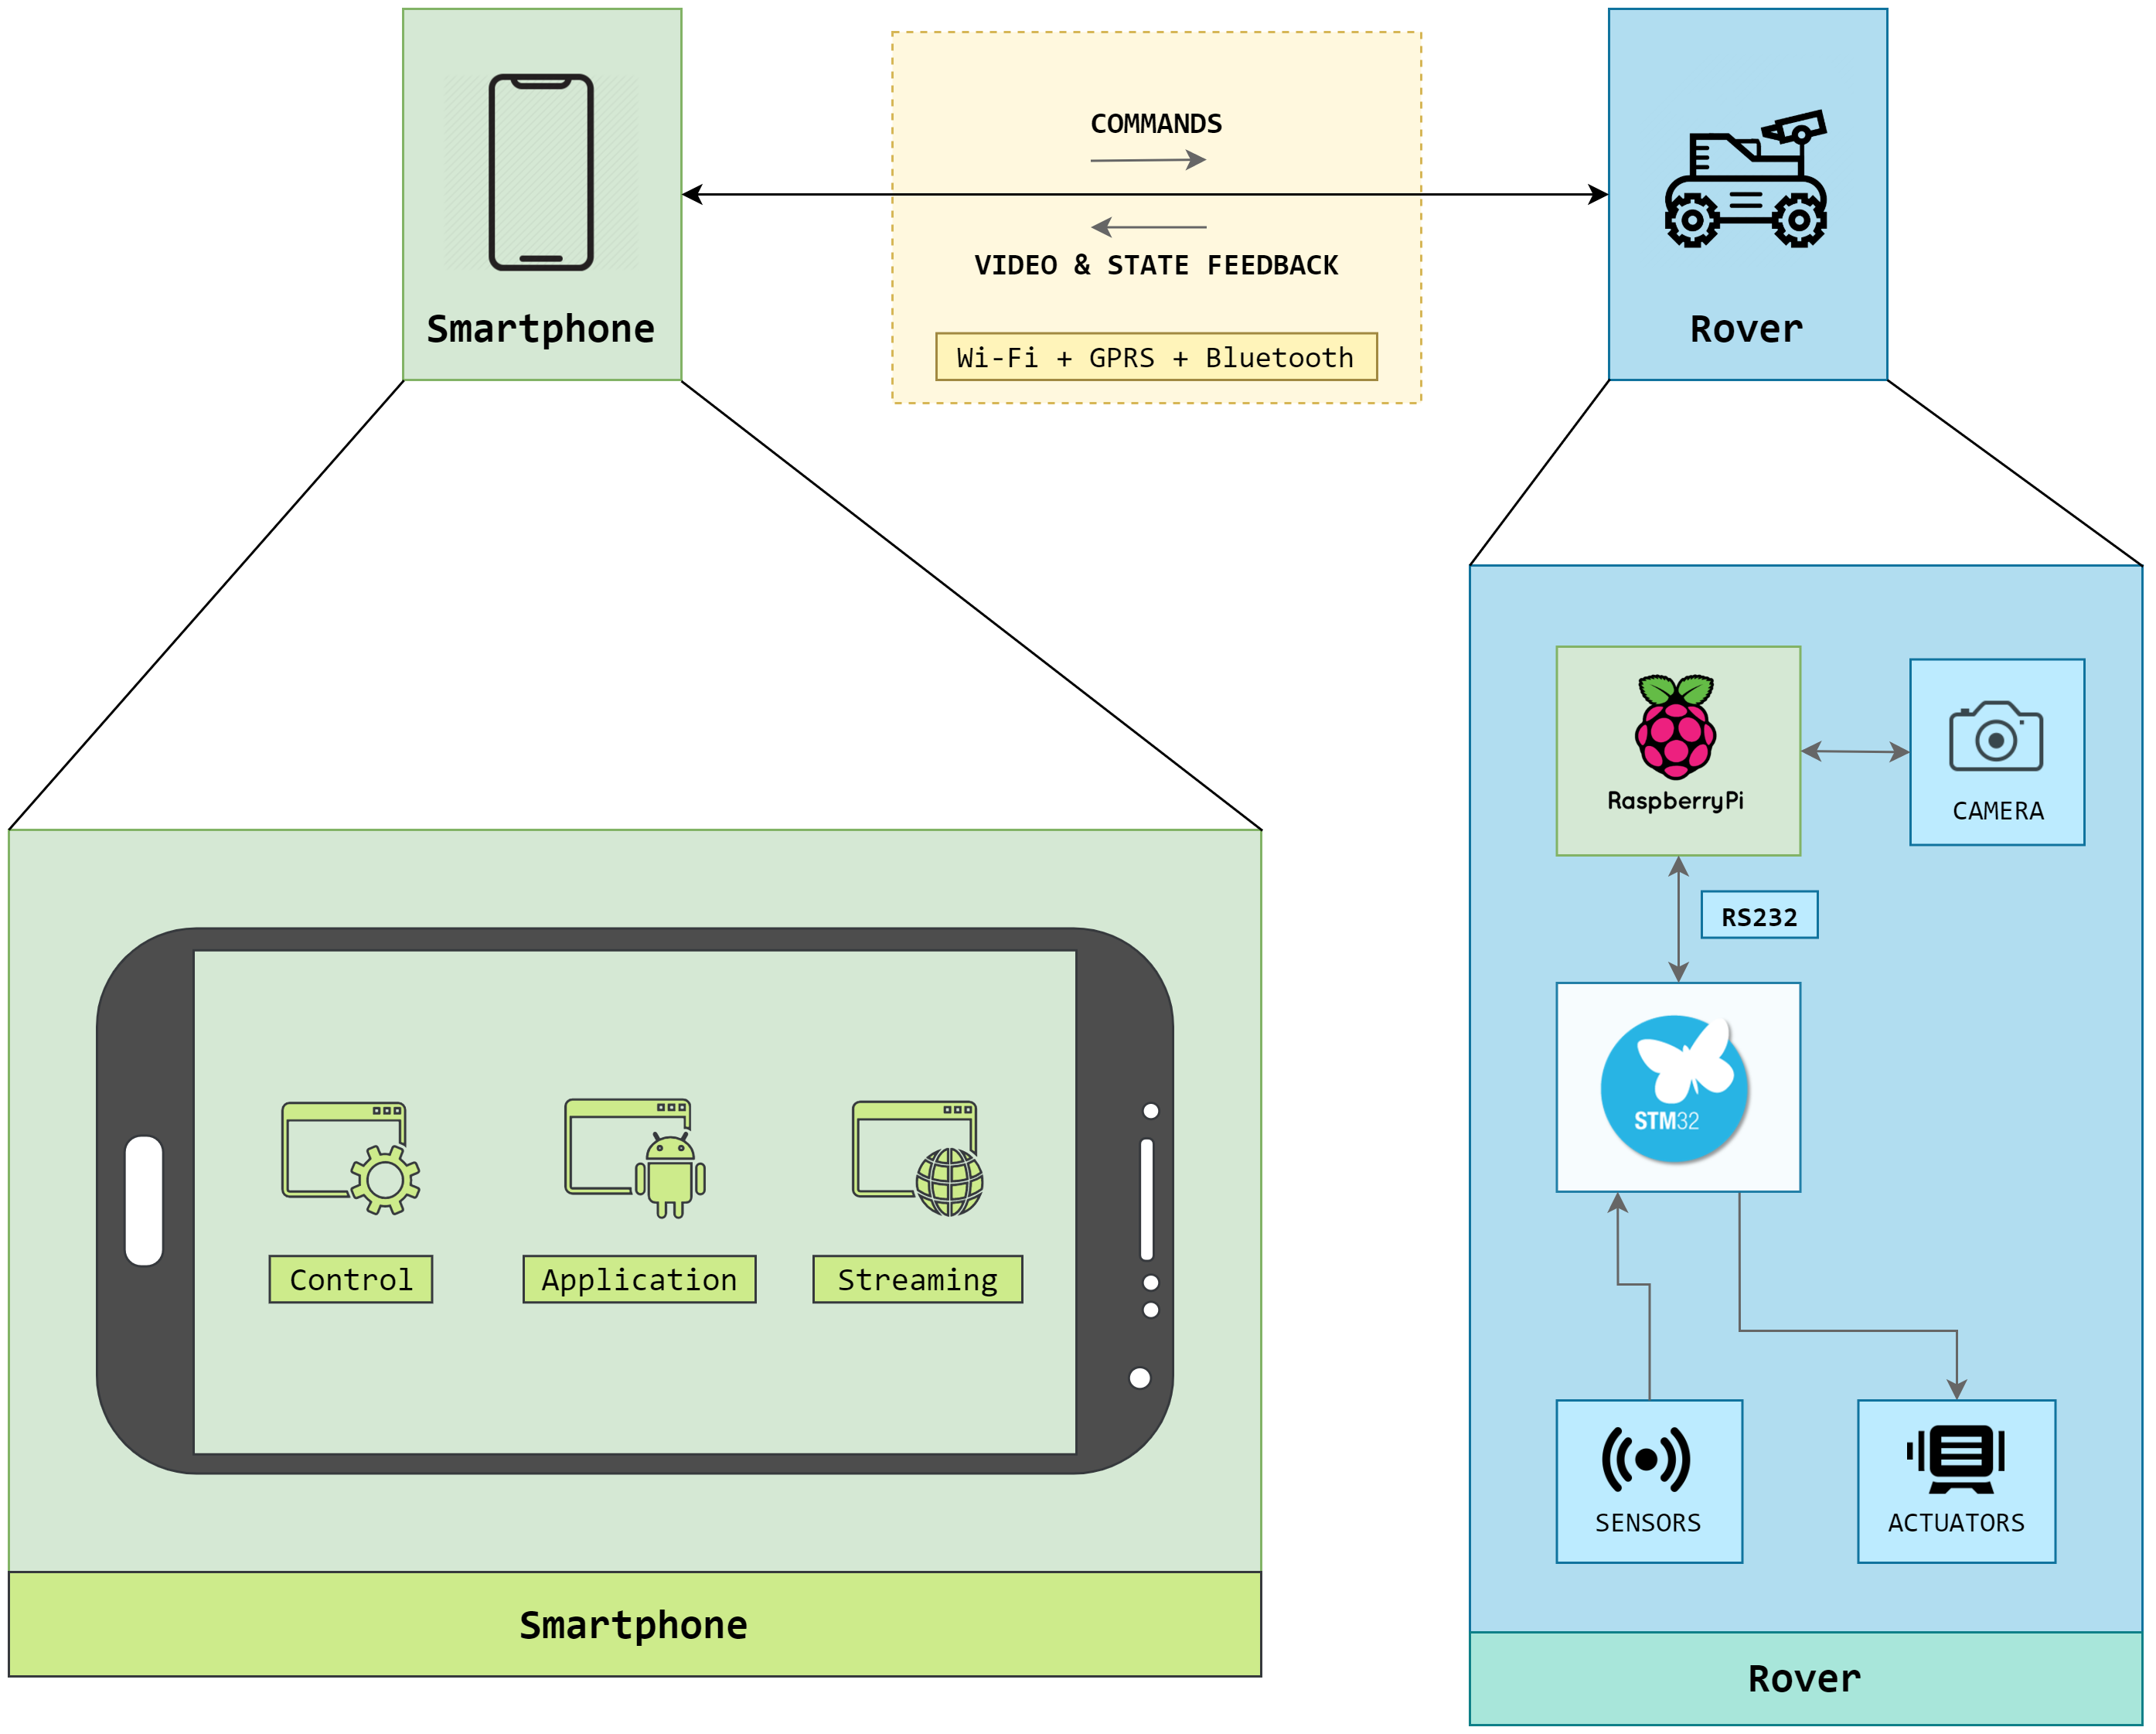
\includegraphics[width=1.0\textwidth]{./img/initial_design_diagram.png}
\caption{\label{fig:initial-design}Initial design: Block diagram view}
\end{figure}
\end{lstlisting}
\textbf{Result} (see Fig. \ref{fig:initial-design}):
\begin{figure}[!ht]
\centering
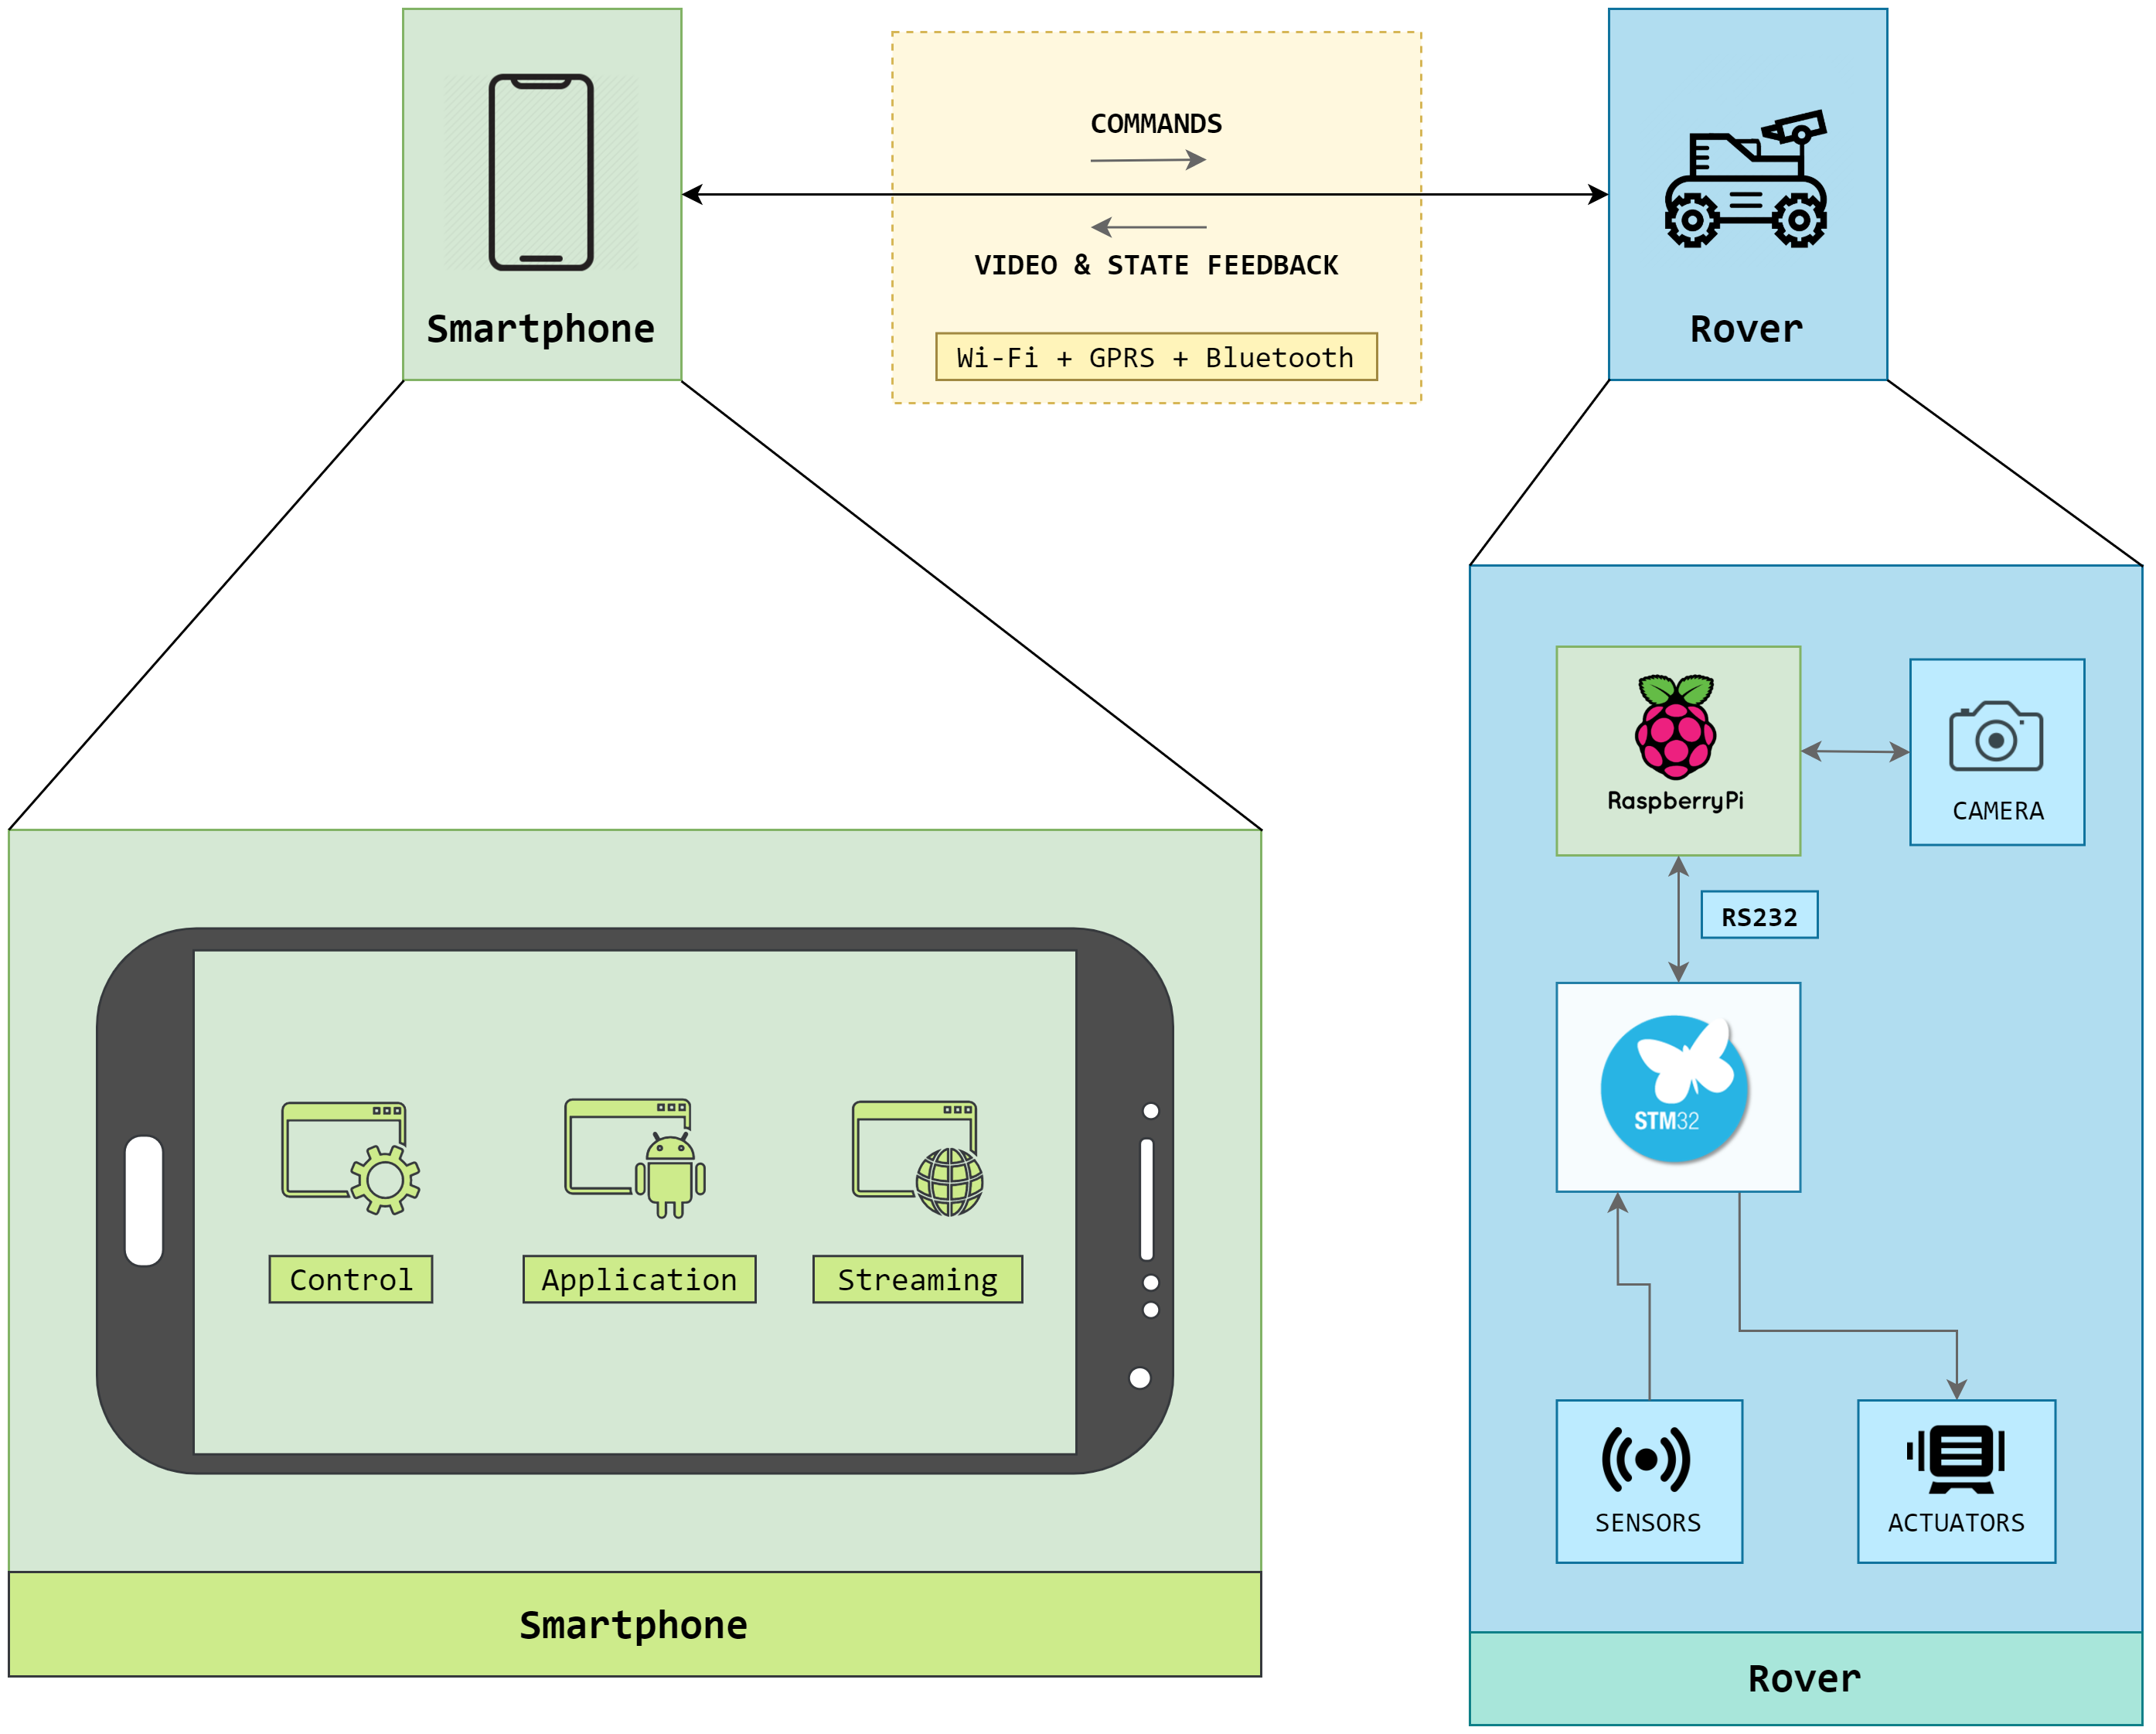
\includegraphics[width=1.0\textwidth]{./img/initial_design_diagram.png}
\caption{\label{fig:initial-design}Initial design: Block diagram view}
\end{figure}
\subsection{Tables}
\label{sec:orgd573a75}
\begin{enumerate}
\item Construction: Tables can be created using an online tool
(\url{https://www.tablesgenerator.com/}) and then copied, as illustrated in
\emph{Definition}
\item Definition: 
\lstset{language=[LaTeX]TeX,label= ,caption= ,captionpos=b,numbers=none}
\begin{lstlisting}
% Please add the following required packages to your document preamble:
% \usepackage[table,xcdraw]{xcolor}
\begin{table}[!hbt]
\centering
\caption{Specifications}%
\label{tab:specs-init}
%
\begin{tabular}{
>{\columncolor[HTML]{FFFFFF}}l 
>{\columncolor[HTML]{FFFFFF}}l 
>{\columncolor[HTML]{FFFFFF}}l }
\hline
		& Values     & Explanation                                                                                                  \\ \hline
Autonomy          & 4 h        & \begin{tabular}[c]{@{}l@{}}Time interval between battery fully \\ charged and safely discharged\end{tabular} \\ \hline
Speed Range  & 0.1 to 1 m/s    & \begin{tabular}[c]{@{}l@{}}Speed at which the car can operate\end{tabular}              \\ \hline
Frame Rate        & 60 fps     & \begin{tabular}[c]{@{}l@{}}Frequency at which independent still \\ images appear on the screen\end{tabular}  \\ \hline
Camera Range      & 20 m       & \begin{tabular}[c]{@{}l@{}}How far can the camera capture images\\ without loosing resolution\end{tabular}   \\ \hline
Camera resolution & 480p       & Amount of detail that the camera can capture                                                                 \\ \hline
Communication Range & 50 m & \begin{tabular}[c]{@{}l@{}}Maximum distance between the car and the\\ smarphone without losing connection\end{tabular} \\ \hline
speed Error    & 5 \%       & \begin{tabular}[c]{@{}l@{}}Maximum difference between desired \\ and real speed\end{tabular}              \\ \hline
Direction Error   & 5\%        & \begin{tabular}[c]{@{}l@{}}Maximum difference between desired\\  and real direction\end{tabular}             \\ \hline
Distance Error     & 5 \% & \begin{tabular}[c]{@{}l@{}}Maximum difference between desired\\ and real distance to the obstacle\end{tabular}         \\ \hline
Dimensions        & 20x12x5 cm & Dimensions of the car                                                                                        \\ \hline
Weight            & 0.5 kg     & Weight of the car                                                                                            \\ \hline
\end{tabular}
\end{table}
\end{lstlisting}
\item \textbf{Result}: Table \ref{tab:specs-init} lists the foreseen product
specifications.
\begin{table}[!hbt]
\centering
\caption{Specifications}%
\label{tab:specs-init}
%
\begin{tabular}{
>{\columncolor[HTML]{FFFFFF}}l 
>{\columncolor[HTML]{FFFFFF}}l 
>{\columncolor[HTML]{FFFFFF}}l }
\hline
		& Values     & Explanation                                                                                                  \\ \hline
Autonomy          & 4 h        & \begin{tabular}[c]{@{}l@{}}Time interval between battery fully \\ charged and safely discharged\end{tabular} \\ \hline
Speed Range  & 0.1 to 1 m/s    & \begin{tabular}[c]{@{}l@{}}Speed at which the car can operate\end{tabular}              \\ \hline
Frame Rate        & 60 fps     & \begin{tabular}[c]{@{}l@{}}Frequency at which independent still \\ images appear on the screen\end{tabular}  \\ \hline
Camera Range      & 20 m       & \begin{tabular}[c]{@{}l@{}}How far can the camera capture images\\ without loosing resolution\end{tabular}   \\ \hline
Camera resolution & 480p       & Amount of detail that the camera can capture                                                                 \\ \hline
Communication Range & 50 m & \begin{tabular}[c]{@{}l@{}}Maximum distance between the car and the\\ smarphone without losing connection\end{tabular} \\ \hline
speed Error    & 5 \%       & \begin{tabular}[c]{@{}l@{}}Maximum difference between desired \\ and real speed\end{tabular}              \\ \hline
Direction Error   & 5\%        & \begin{tabular}[c]{@{}l@{}}Maximum difference between desired\\  and real direction\end{tabular}             \\ \hline
Distance Error     & 5 \% & \begin{tabular}[c]{@{}l@{}}Maximum difference between desired\\ and real distance to the obstacle\end{tabular}         \\ \hline
Dimensions        & 20x12x5 cm & Dimensions of the car                                                                                        \\ \hline
Weight            & 0.5 kg     & Weight of the car                                                                                            \\ \hline
\end{tabular}
\end{table}
\end{enumerate}
\section{Referencing}
\label{sec:org4434181}
To reference the relevant items such as figures, tables, sections (chapter,
section, subsection), etc., one needs:
\begin{enumerate}
\item To label the item, using \texttt{\textbackslash{}label\{<item>:<item-name>\}}:
e.g. \texttt{\textbackslash{}label\{ch:analysis\}}
\item Then, one can reference it using: \texttt{\textbackslash{}ref\{<item>:<item-name>\}}:
e.g. Chapter\textasciitilde{}\ref{ch:analysis}
\end{enumerate}
\section{Bibliography}
\label{sec:orge62b455}
Bibliography management is composed of 2 parts:
\begin{enumerate}
\item A Bibliography database, generally a \texttt{.bib} file, located at
\texttt{./bib/dissert.bib} (see \href{file:///Users/zemiguel/Documents/Univ/MI\_Electro/Sem6/LPI2/PI/github/Deliverables/Final/bib/dissert.bib}{here})
\begin{itemize}
\item Example of Bibliography entry
\lstset{language=[LaTeX]TeX,label= ,caption= ,captionpos=b,numbers=none}
\begin{lstlisting}
@article{harashima1996mechatronics,
  title={Mechatronics-" What Is It, Why, and How?" An Editorial},
  author={Harashima, Fumio and Tomizuka, Masayoshi and Fukuda, Toshio},
  journal={IEEE/ASME Transactions on Mechatronics},
  volume={1},
  number={1},
  pages={1--4},
  year={1996},
  publisher={IEEE}
}
\end{lstlisting}
\item Bibliography entry can be created as:
\begin{itemize}
\item Search the topic at \url{https://scholar.google.pt/}.
\item Select the Export To Bibtex option
\item Copy to the \texttt{.bib} file
\end{itemize}
\end{itemize}
\item A citation, using \texttt{\textbackslash{}cite\{<bib-key>\}}, where \texttt{<bib-key>} is the key defined in
the \texttt{.bib} file. 
\begin{itemize}
\item For example: Mechatronics, was defined by Harashima
et. al=\textasciitilde{}\cite{harashima1996mechatronics}=
\end{itemize}
\end{enumerate}
\section{Enviroments}
\label{sec:org4102c27}
\subsection{Itemize}
\label{sec:org574551c}
\lstset{language=[LaTeX]TeX,label= ,caption= ,captionpos=b,numbers=none}
\begin{lstlisting}
\begin{itemize}
\item \textbf{Item 1}: this is an item
\item \textbf{Item 2}: this is another item
\end{itemize}
\end{lstlisting}
\textbf{Result}:
\begin{itemize}
\item \textbf{Item 1}: this is an item
\item \textbf{Item 2}: this is another item
\end{itemize}

\subsection{Enumerate}
\label{sec:org9d11cf3}
\lstset{language=[LaTeX]TeX,label= ,caption= ,captionpos=b,numbers=none}
\begin{lstlisting}
\begin{enumerate}
\item \textbf{Item 1}: this is an enumerated item
\item \textbf{Item 2}: this is another enumerated item
\end{enumerate}
\end{lstlisting}
\textbf{Result}:
\begin{enumerate}
\item \textbf{Item 1}: this is an enumerated item
\item \textbf{Item 2}: this is another enumerated item
\end{enumerate}
\section{Glossary}
\label{sec:org8845f59}
Glossaries are useful to input \uline{acronyms} and \uline{symbols}.
\begin{itemize}
\item Acronyms: common use words, often abbreviated.
\item Symbols: mathematical/physical symbols that usually require some brief
description and the relevant units.
\end{itemize}

Glossary management is composed of 3 parts:
\begin{enumerate}
\item A Glossary database 
\begin{itemize}
\item Acronyms: \texttt{./sec/acronyms.tex}
\item Symbols: \texttt{./sec/symbols.tex}
\end{itemize}
\item A reference using \texttt{\textbackslash{}gls\{<gls-key>\}}, where \texttt{<gls-key>} is the key defined in
the glossary database file.
\item An external utility that manages the glossary entry items addition and
referencing (no need to worry about this, the makefile will handle it).
\end{enumerate}
\subsection{Acronyms}
\label{sec:orgc5e2914}
\begin{itemize}
\item Definition (\texttt{./sec/acronyms.tex}):
\lstset{language=[LaTeX]TeX,label= ,caption= ,captionpos=b,numbers=none}
\begin{lstlisting}
\newacronym{sls}{SLS}{Selective Laser Sintering}
\newacronym{slm}{SLM}{Selective Laser Melting}
\end{lstlisting}
\item Usage: These are two acronyms used together: \texttt{\textbackslash{}gls\{sls\}/\textbackslash{}gls\{slm\}} technology.
\end{itemize}

\subsection{Symbols}
\label{sec:orgd66ae0b}
\begin{itemize}
\item Definition (\texttt{./sec/symbols.tex}):
\lstset{language=[LaTeX]TeX,label= ,caption= ,captionpos=b,numbers=none}
\begin{lstlisting}
\newglossaryentry{omega}
{
    name={\ensuremath{\omega}},
    description={angular velocity},
    sort=omega,
    symbol={\ensuremath{\omega}},
    unit={\si{rad/s}}
}
\end{lstlisting}
\item Usage: this is \texttt{\textbackslash{}gls\{omega\}}.
\end{itemize}

\section{Listings}
\label{sec:org52673a7}
\begin{itemize}
\item Styling: Listings can be formatted using different styles, as presented in
\texttt{./sty/listing.sty} for any programming/markup language required.
\begin{itemize}
\item Example: C
\lstset{language=[LaTeX]TeX,label= ,caption= ,captionpos=b,numbers=none}
\begin{lstlisting}
\lstdefinestyle{customc}{
belowcaptionskip=1\baselineskip,
breaklines=true,
%frame=L,%lines, whole
xleftmargin=\parindent,
language=C,
showstringspaces=false,
basicstyle=\scriptsize\ttfamily,
keywordstyle=\bfseries\color{green!40!black},
commentstyle=\itshape\color{purple!40!black},
identifierstyle=\color{blue},
stringstyle=\color{orange},
numberstyle={\tiny},
numbers=left,
numberblanklines=false,
stepnumber=5,
backgroundcolor=\color{yellow!10}, 
frame=tlb
}
\end{lstlisting}
\end{itemize}
\item Usage: Listings can be inputted using the desired style as below. It includes
a caption, a label, a style, and a file path:
\lstset{language=[LaTeX]TeX,label= ,caption= ,captionpos=b,numbers=none}
\begin{lstlisting}
\lstinputlisting[language=C++, caption={Thread Serial Rx handler},label=lst:threadSerialRx,
style=customc]{./listing/threadSerialRx.cpp}%
\end{lstlisting}
\item Result:
\end{itemize}
\lstset{language=C,label= ,caption= ,captionpos=b,numbers=none,style=customc}
\begin{lstlisting}
UINT MMSLSDlg::ThreadSerialRx(LPVOID param)
{
    /* Wait for 1st connection to serial port: OnConnect */
    ::WaitForSingleObject( EvSerial.m_hObject , INFINITE); 
    tstring szData;
    CDemoEzdDlg *dlg = (CDemoEzdDlg *)param;

    while(1)
    ;

    return 0;
}
\end{lstlisting}
\section{PDF inclusion}
\label{sec:orgd6f8882}
\begin{itemize}
\item Include all pages from \texttt{anexo3-license}. Be careful of file path. It's
relative to the main file.
\lstset{language=[LaTeX]TeX,label= ,caption= ,captionpos=b,numbers=none}
\begin{lstlisting}

\includepdf[pages=-]{anexo3-license}
\end{lstlisting}
\end{itemize}
\section{Appendices}
\label{sec:org8624020}
Appendices can be added in the appropriate section (\texttt{./tex/Append/}):
\begin{itemize}
\item as text: with figures, tables, etc.
\item included as PDF
\end{itemize}
\end{document}